% To translators: don't bother to translate this... english-only version.

Advertisement.

Occasionally I do \href{https://en.wikipedia.org/wiki/Software_protection_dongle}{software copy-protection dongle} replacements or dongle emulators.

Like this ancient LPT dongles (newer dongles are almost like USB sticks):

\begin{figure}[H]
\centering
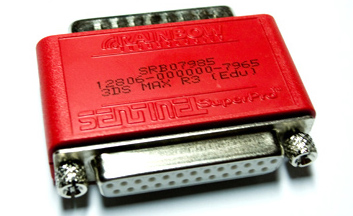
\includegraphics[width=0.5\textwidth]{superpro.jpg}
\end{figure}

In general, it is somewhat unlawful to break software protection, so I can do this only if these conditions are met:

	\begin{itemize}
	\item the software company who developed the software product does not exist anymore to my best knowledge;
	\item the software product is older than 10 years;
	\item you have a dongle to read information from it. In other words, I can only help to those who still uses some very old software, completely satisfied with it, but afraid of dongle electrical breakage and there are no company who can still sell the dongle replacement.
	\end{itemize}

These includes ancient MS-DOS and UNIX software. Software for exotic computer architectures (like MIPS, DEC Alpha, PowerPC) accepted as well.

Examples of my work you may find in this book.

Typical price is USD 300.

E-Mail: \EMAIL{}, Skype: dennis.yurichev, Telegram: \TT{@yurichev}.

